\newcommand{\NOTEHERE}[1]{\colorbox{yellow}{\textcolor{blue}{
    \lparen\lparen\lparen}\textcolor{
        red}{#1}\textcolor{blue}{\rparen\rparen\rparen}}}

% newline
\newcommand{\PROBABLY}[1]{}
%% \newcommand{\PROBABLY}[1]{\colorbox{red}{\textcolor{green}{
%%     \lbrack\lbrack\lbrack}\textcolor{green}{#1}\textcolor{
%%         green}{\rbrack\rbrack\rbrack}}}

% \textcolor{green}{#1}
\newcommand{\FIXTHIS}[1]{\par\makebox[\textwidth]{
    \colorbox{pink}{\textcolor{green}{
        \lbrack\lbrack\lbrack}\textcolor{
            blue}{#1}\textcolor{green}{\rbrack\rbrack\rbrack}}}}

\newcommand{\mysetcounter}[2]{\setcounter{#1}{\the\numexpr#2 - 1\relax}}
\newcommand{\mychcnt}[1]{\mysetcounter{chapter}{#1}}
% \newcommand{\mychcnt}[1]{}

\newcommand{\mysccnt}[1]{\mysetcounter{section}{#1}}

% \newcommand{\CITEME}{\colorbox{red}{\textcolor{green}{
%     \lparen\lparen\lparen}\textcolor{
%         white}{CITEME\textcolor{green}{\rparen\rparen\rparen}}}\:}
\newcommand{\CITEME}{\colorbox{red}{\textcolor{green}{
    \lparen}\textcolor{
        white}{?\textcolor{green}{\rparen}}}\:}

\newcommand{\mycite}[1]{[\textcolor{red}{#1}]}
\newcommand{\uucite}[1]{[\textcolor{red}{\footnote{#1}}]}
\newcommand{\citetag}[1]{}
\newcommand{\myhline}{\noindent\makebox[\linewidth]{\rule{\paperwidth}{0.4pt}}}

\newcommand{\draftbegin}{\centerline{\textcolor{magenta}{\textbf{=======================以下是草稿!=======================}}}}
\newcommand{\drafttermi}{\centerline{\textcolor{blue}{\textbf{=======================以上是草稿!=======================}}}}


%%%%%%%%%%%%%%%%%%%%%%%%%%%%%%%%%%%%%%%%%%%%%%%%%%%%%%%%%%%%%%%%%%%%%%%%%%%%%%%%

{\mysinglespacing\selectfont
% \tableofcontents
\par}
\newpage\setcounter{page}{1}\pagenumbering{arabic}

\newcommand{\jeffcomment}[1]{}

% \chapter{導論}

\section{研究動機}
  
語言是人與人彼此交流最主要的橋樑,而人們互相溝通最自然的方式便是透過說話的語音(Speech)達成。人類往往是自幼就牙牙學語開始說話,直到已屆學齡左右才開始學習認字與書寫。雖然在這個資訊爆炸的時代,人們已經習慣以文字呈現的語言作為獲取資訊的主要媒介,但不論如何,各種書寫系統其背後承載的語言必定有語音的形式作為對應。更何況世界上現存大約七千多種 \cite{eberhard_ethnologue_2024} 語言中,絕大多數不見得存在成熟且普及的文字系統,卻無礙於這些語言被人們所熟悉和使用。因此,「語音」作為語言不可或缺的存在方式,了解它和研究它的價值自然不言而喻。

然而,相對於穩定、易於處理和保存的文字文本,語音訊號的變化萬千,蘊藏了大量從語者風格、表達內容到抑揚頓挫(韻律,Prosody)等不同層次的訊息,使得對它的處理、研究相比之下複雜度與難度劇增。由於語音的這種特性,過往對於語言最有興趣的語言學家們,即便明白語音作為多數語言主體的事實,也不得不藉文字符號為依託進行探索。進入資訊化時代後,藉助電腦硬體等計算設備的幫助,從語料庫、計算語言學到自然語言處理等透過科技的力量發展語言處理技術的領域,頗長一段時間也是專注於文字的處理與分析。
而嘗試結合訊號處理發展的語音技術領域,當時則是透過語言學家對語言的領域知識,例如從音位(Phoneme)、構詞(Morphology)、語法(Syntax)等等用以刻劃人類語音和語言特性的概念,將之結合機器學習建立模型,開發技術以方便人們能以語音這種更靈活的媒介,更好的讓電腦、手機等科技工具可以更接近「直接溝通」的使用方式,便利人們的日常生活。

近年來,由於圖形處理器(Graphics Processing Unit,GPU)等硬體平行運算技術的進步,深層學習(Deep Learning)快速崛起成為人工智慧的主流,有了此項機器學習的技術,模型的彈性能夠更好的萃取資料、更貼近的尋找資料背後的機制並進行預測,使得人們不再非得依賴大量費時費工的人類標注過程,進而使得利用大量語料庫發展語言技術,進一步推進語言科技發展成為可能。尤其在自監督學習(Self-supervised Learning)技術出現之後,深層學習模型可以依照人們給定的方向,更細緻的從大量未標注、相較容易取得的語音或文字的語料,找出其中的語音、語法及語義等等結構,形成帶有對人類語言有前所未見表現的基石模型(Foundation Model),是這個領域的一大里程碑。尤其在以處理文字為主體的自然語言處理領域,甚至出現了幾乎使人類真偽難辨的生成式模型,改變了人們生活的方方面面。

借鏡文字方面的成功經驗,語音處理領域的研究者們也開始嘗試將語言模型(Language Model)的概念套用於變化莫測的語音訊號之上,原先人們藉助訊號處理知識一直使用的各種語音訊號特徵(Feature)也在自監督學習的架構之下,出現了許多模型從大量語音資料中得到的「語音表徵(Speech Representation)」,作為精煉語音資訊的另外一種新選擇開始廣泛被採用。然而,相比於文字符號的穩定與單純,語音的複雜性使得它處理起來會需要更大量的資料和運算資源來擷取其中不同層次的細節,而且作為物理訊號,語音還必須處理掉環境中的雜訊等干擾。為了從紛亂的聲音中提取出最重要的訊息,向量量化(Vector Quantization)的技巧因而經常被使用在語音 \cite{chorowski_unsupervised_2019,chen_vector_2023,zhao_speech_2023} 或影像的領域中。爾後, \cite{lakhotia_generative_2021-1}  基於模仿人類學習語言的過程,藉助諸如 CPC(\cite{oord_representation_2019} )、HuBERT (\cite{hsu_hubert_2021} )、wav2vec 2.0 (\cite{baevski_wav2vec_2020} )等自監督學習模型的幫助,引入向量量化的技術,提出了「無文字(Textless)」的學習架構,轉而以語音表徵量化後的「離散單元(Discrete Unit)」作為操作對象,企圖以單純大量的語音資料中訓練出一個不依賴文字的語言模型。此種學習架構的優勢在於在能保有利用大量未標注文字轉寫語音資料的同時,與連續表徵相比資訊的位元率(Bit Rate)利用更有效率、容易儲存、處理與傳輸,以及形式上更像文字的特性,因而可以將其視為一種「機器自己學習出來的文字」,接下來借用長久以來只能在自然語言處理(Natural Language Processing,NLP)領域中各種語言模型(Language Model)的相關技術和任務的解決方法,套用在語音處理的領域中,期望可以像文字那樣從大量的語音資料中,找尋出「語音訊號版本的文字」。自此之後有一系列如應用於英語和閩南語之間的語音到語音翻譯 \cite{chen_speech--speech_2023} 等等使用離散單元(Discrete Unit)進行任務訓練的研究,一定程度的印證了這些離散單元捕捉語音內容的效果。

儘管離散單元在編碼語音之上固然有不錯的效果,並有相關研究展現了離散單元具有一定程度上與文字的相似性,然而其作為「完全文字的替代」仍然有相當的距離。借鑑過往在自監督學習的語音表徵出來之後,便嘗試重新從語言學(Linguistics)的概念汲取靈感,對其進行語音學(Phonetics)層面的分析。本論文期望初步結合原先 HuBERT 中從消息理論(Information Theory)的統計數據,結合語音學分析的視角,對於離散表徵(Discrete Representation)本身與音位(Phoneme)和語音類別(Phone Type)之間的關係進行相關性的統計與分析,期望可以對 HuBERT 等自監督學習表徵進行量化(Quantization)後所得的離散單元所編碼、擷取到的資訊是什麼有較為深入程度的了解。


% 直接快速帶過連續的 Speech Repr
% Acoustic Piece 那邊的文獻到後面再寫。到這裡已經夠承先啟後了
    
\section{研究方向}
  
本研究論文為了探究離散單元本身是否具有潛力可以單純透過大量語音資料的自監督學習與統計過程,從文本中找尋出語音中更精細的結構,乃至於類似文字或是從語言學(Linguistics)等人類知識領域定義出的「離散單位」 --- 如音素(Phone)、音位(Phoneme)、字符(Character)、「詞綴與字根」(即「詞素(Morpheme)」)或單字(Word)等等。因此,本研究取法自 HuBERT 本身為了證明其離散單元具有一定的「聲學單元(Acoustic Unit)」特性的「純度(Purity)」和「相互資訊(Mutual Information,MI)」的分析數據作為分析離散語音表徵和「音位」 --- 作為人類知識理解語音中最基礎的單位 --- 之間相關性(Correlation)的參考。

此外,基於訊號速率(如序列的長度)的考量,結合在文字處理中如 BPE 等等常見的次詞單位(Subword)分詞(Tokenization)演算法,基於形式上的相似性,因而也可以套用在像是 HuBERT離散單元這種離散的符號上,將離散單元序列中相似的規律(Pattern)發掘出來。近期如 Wav2Seq \cite{wu_wav2seq_2023}、\cite{ren_speech_2022}、\cite{chang_exploring_2024} 等作品也先進行了類似的嘗試。本論文則是在除了經驗上(Empirically)將其用於大量資料訓練的視角以外,從「將其視為另一種離散單位」的觀點進行統計數據的量化分析(Quantitative Analysis),作為在計算資源有限的前提下決策數據編碼的一個判斷標準。

\section{主要貢獻}
  
本論文達成的主要成果是以更細緻的方式,對現在愈來愈廣為使用的離散單元以音位和語音類別等語音知識的視角給出一個基礎相關性的分析方法,並將單一離散單元本身與將多個單元透過分詞演算法(Tokenization)重新編碼前後進行比較,初步試探離散單元與音位之間的關係,並期望作為「離散單元 可否一定程度上的『被視為文字』或『有機會從中發掘出文字單位』」的判斷基礎,為往後研究往語音語言模型(Spoken Language Model)中「對語音編碼」這個重要的程序,提供一個在實際上開始耗費資源的模型訓練之前,可比較的判斷標準。

\section{章節安排}

本論文將以如下的方式進行章節安排:

\begin{itemize}
  \itemsep -2pt %reduce Space Between Items
  \item  第二章:介紹後面章節所需要的與深層學習(Deep Learning)、表徵學習與自監督學習相關的基礎背景知識。
  \item  第三章:從介紹離散單元本身提出後,「無文字」的相關前作文獻開始,帶出對從無文字系列作品用到的各種自監督學習模型抽取之離散單元本身的純度(Purity)和相互資訊(Mutual Information,MI)等統計數據,進行比較與分析。
  \item  第四章:講述為何單一離散單元本身或許不全然足夠發掘出類似音位進而對應到文字的單位,以及近年人們嘗試以離散單元為基礎,透過分詞演算法(Tokenization Algorithm)發展之聲學片段(Acoustic Piece) 的進展,接著我們將單元進行分詞法重新編碼處理前後,觀察數據上與第三章結果間的差異,以論證對離散單元進行分詞是否可以找出更接近音位的單位,驗證「離散單元可被文字化」或「離散單元學到的是否為更精細的語音訊號規律或結構(Structure)」等論述。
  \item  第五章:總結前面的觀察結果,並進一步探討本研究還可以如何延伸,並怎麼幫助語音語言模型的發展。
\end{itemize}

% \mychcnt{2}  %
% 
\chapter{背景知識}

\section{深層類神經網路}

\subsection{簡介}

  深層類神經網路(Deep Neural Network,DNN)是由神經科學家麥氏(McCulloch)與皮氏(Pitts)於 1943 年提出 \cite{mcculloch_logical_1943} 的計算模型,靈感取自連結主義(Connectionism)的核心主張 --- 以模仿生物神經網路的連結方式模擬複雜的心智活動。

        為模擬神經細胞處理訊號的過程,深層類神經網路最基本的單位稱為「神經元(Neuron)」,其本質為線性分類器。每個神經元接收的輸入數值 $x = (x_1, x_2, \cdots\cdots, x_N)$ 是一個 $N$ 維向量,每一維會被賦予一個權重(Weight) $w = (w_1, w_2, \cdots\cdots, w_N)$  ,加權後總和再加上偏差值 $b$,得到線性輸出值。為了模擬神經細胞的觸發過程,該分類器常被加上非線性的激發函數(Activation Function)$\sigma$ 的轉換,才得到最終輸出值 $y$。如圖 \ref{fig:single-neuron}所示,神經元的運算規則以下列數學式描述:
\begin{align}
    y = \sigma(w^T x + b)
\end{align}
常見的激發函數包含線性整流單元(Rectified Linear Unit,ReLU)、S 函數(Sigmoid Function)或雙曲正切函數(Hyperbolic Tangent Function,$\tanh$)等等。

\begin{figure}
    \centering
    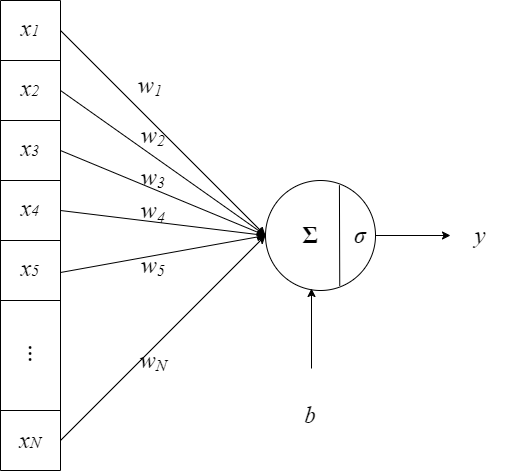
\includegraphics[width=0.5\linewidth]{figures/neuron.drawio.png}
    \caption{神經元示意圖}
    \label{fig:single-neuron}
\end{figure}

        結合數個神經元的運算,羅氏(Rosenblatt)於 1958 年 \cite{rosenblatt_perceptron_1958} 提出感知器(Perceptron)模型。根據通用近似定理(Universal Approximation Theorem)\cite{funahashi_approximate_1989} ,感知器理論上可逼近任意函數。然而,後續研究發現單層的感知器具有如「線性不可分」\footnote{例如無法貼合異或(Exclusive OR,XOR)運算等函數} 等先天限制,使其曾經一度不被看好。

        為了突破該缺陷,人們嘗試在輸入與輸出層之間增加「隱藏層(Hidden Layer)」,成為「多層感知器(Multilayer Perceptron,MLP)」,如圖 \ref{fig:mlp} 所示。藉助隱藏層的幫助,多層感知器可對輸入進行多次非線性轉換,大大拓展了模型的適用範圍。此模型是透過「加深隱藏層」得來,現今為人們熟知的「深層類神經網路(Deep Neural Network)」即由此得名。

\begin{figure}
    \centering
    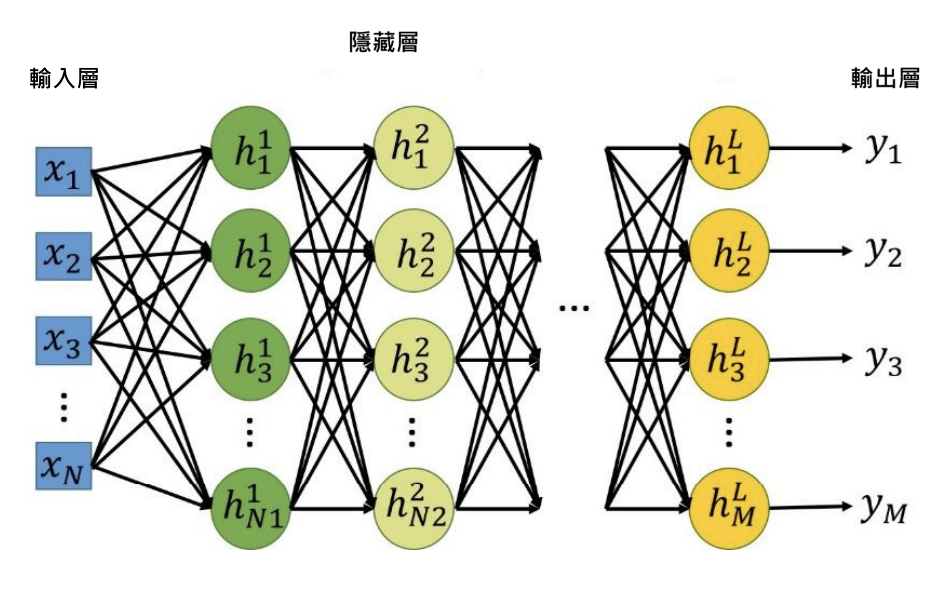
\includegraphics[width=0.8\linewidth]{figures/nnout.png}
    \caption{多層感知器/深層類神經網路示意圖}
    \label{fig:mlp}
\end{figure}

        % 確認那個「大量」跟「應用」有沒有掉字
        藉助深層類神經網路的彈性,我們可以透過大量訓練資料來訓練模型,藉此逼近應用任務中欲近似的函數 $f$,該函數蘊藏在資料集 $\mathcal{D} = \{(x_i, y_i)\}_{i=1}^N$ 中,其中每個資料點 $(x_i, y_i)$ 為輸入與輸出間的配對,即對於 $N$ 個資料點都有 
\begin{align}
    y_i = f(x_i) \ \  \forall i \in \{1, \cdots\cdots, N\}
\end{align}
之關係。為了使這個函數更加逼近目標函數 $f$,類神經網路會構建一個逼近中的函數 $f_{\theta_t}(\cdot)$ 。透過不停的迭代,模型對資料集 $\mathcal{D}$ 的每一筆資料 $x$ 給出預測 $f_{\theta_t}(x)$ 。透過某個減損函數(Loss Function)$\mathcal{L}$ 計算出誤差(Error),此誤差對參數 $\theta_t$ 求出梯度(Gradient)後將指示模型更新的方向,以此乘上學習率(Learning Rate)$\eta$ 後從參數  $\theta_t$ 減去,便能對整個模型進行更新,使之更有機會接近目標函數 $f$。由於此過程是依照梯度使得函數 $\mathcal{L}$ 逐步降低,以此獲名「梯度下降法(Gradient Descent)」,其公式如下:
\begin{align}
    \theta_{t+1} \leftarrow \theta_{t} - \eta \nabla_\theta\mathcal{L}(\mathcal{D}, f_{\theta_t}(\cdot))
\end{align}
其中,$t$ 為當前的迭代數,$\theta_t$ 為當前模型參數,$\theta_{t+1}$ 為更新後的模型參數。

        在此模型更新的過程中,減損函數承擔著指引模型逼近的角色,因此根據應用的任務不同,常見的減損函數包括
\begin{itemize}
    \item 均方誤差(Mean Squared Error,MSE):一般用於迴歸(Regression)問題,直接計算兩數值之間的差距的平方和
          \begin{align}
              \mathcal{L}_{\text{MSE}}(y_i, \hat{y}_i) = \frac{1}{N} \sum_{i=1}^{N} (y_i - \hat{y}_i)^2
          \end{align}
          \textcolor{red}{\(\hat{y}_i\) 是……??????????}
    \item 交叉熵(Cross-entropy,CE):一般用於分類(Classification)問題,著重計算兩個機率分佈之間的差異
          \begin{align}
              \mathcal{L}_{\text{CE}}(y_i, \hat{y}_i) = - \sum_{i=1}^{N} \left[ y_i \log(\hat{y}_i) + (1 - y_i) \log(1 - \hat{y}_i) \right]
          \end{align}
\end{itemize}

        透過上述的訓練方式可以得知,類神經網路的訓練需要相當龐大且複雜的運算過程,因此剛提出時仍舊難以應用於現實應用中。

        為了提高函數貼合的效率,魯氏(Rumelhart)與辛氏(Hinton)等人 \cite{rumelhart_learning_1986, rumelhart_learning_1987} 提出了反向傳播(Backpropagation)演算法,旨在將上述的更新過程,藉助鏈鎖率(Chain Rule)的幫助,由隱藏層逐層反向傳播至輸入層,對整個類神經網路進行修正。

        反向傳播演算法的設計,正好能配合圖形處理器(Graphics Processing Unit,GPU)等硬體裝置的優勢,以平行運算能力加速函數貼合(Fit)的效率。由此開始,這種透過深層類神經網路,從大量資料集中發掘函數關係的機器學習演算法,被稱為深層學習(Deep Learning)。 類神經網路在各個領域的泛化能力(Generalizability)已經得到前所未有的效能,包含電腦視覺、語音處理和自然語言處理,因此深層學習在近年成為人工智慧發展的主流。

        然而,根據資料特性的不同,並不是所有的資料都適用簡單的「輸入與輸出配對」的模式。研究者根據任務需求,發展出了不同架構的類神經網路以適應資料特性。前述最基本的深層類神經網路,由於資料是直接由輸入層,通過逐層的矩陣運算得到輸出,因此被稱之為「前饋式類神經網路(Feed Forward Network,FFN)」。

        藉由調整各神經元之間的連接關係,發展出卷積式(Convolutional)、遞迴式(Recurrent)與轉換器(Transformer)類神經網路等架構變體,以適應如影像、語音和文字等不同型態的資料。這些架構在語音與文字處理被普遍使用,接下來將逐一分別介紹:

\subsection{卷積式類神經網路}

  卷積式類神經網路(Convolutional Neural Network,CNN)為 1998 年由楊氏(LeCun) \cite{lecun_gradient-based_1998} 提出,旨在以訊號處理的卷積(Convolution)運算,模擬生物的視覺皮質感知 \cite{hubel_receptive_1959} 。

\begin{figure}
    \centering
    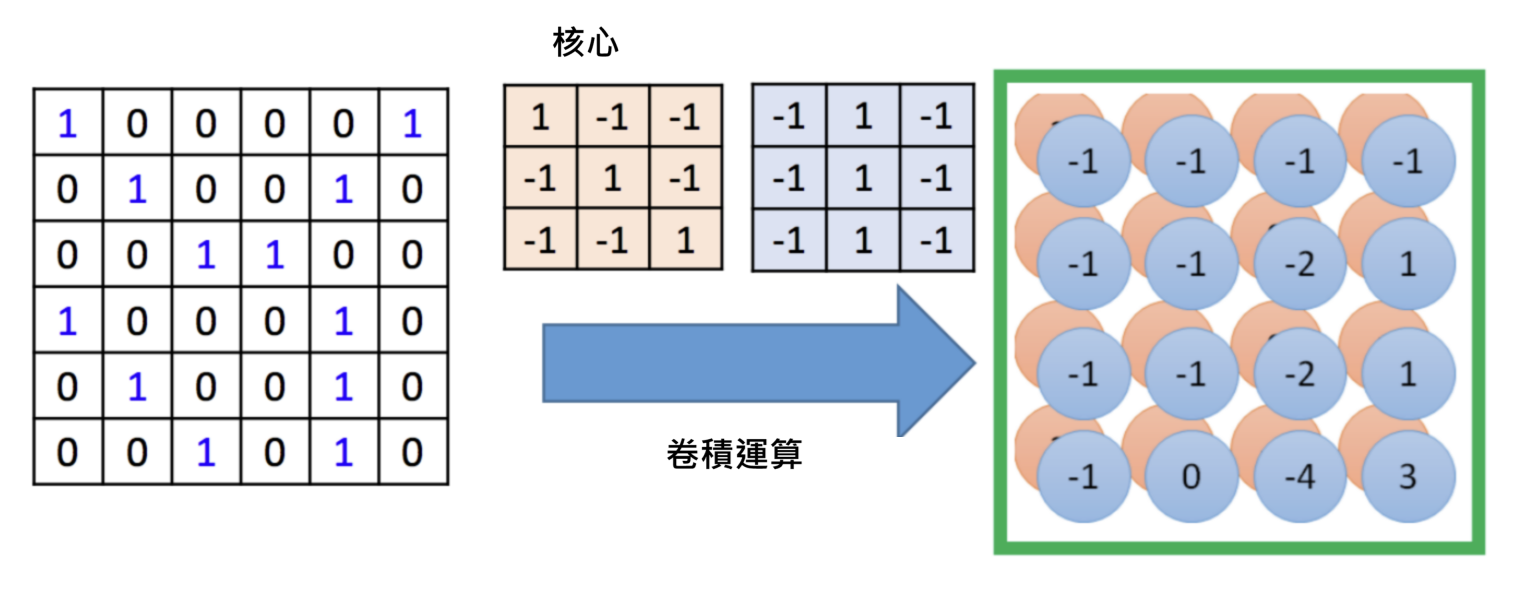
\includegraphics[width=0.9\linewidth]{figures/cnnnew.png}
    \caption{卷積式類神經網路示意圖,取自李宏毅教授的課程投影片}
    \label{fig:cnn}
\end{figure}

        如圖 \ref{fig:cnn} 所示,卷積式類神經網路透過核心(Kernel),對輸入的資料 --- 如圖中的二維矩陣 --- 進行卷積運算,獲得該輸入的特徵圖(Feature Map)。核心帶來的移動不變性(Shift-invariance)非常適用於捕捉二維影像中的局部特徵,以作為類神經網路分辨資料的依據。

        有別於影像處理中,資料多以二維矩陣表示像素 (Pixel)三原色的亮度數值,因此以二維的卷積運算為主;由於語音時常處理時間軸之上的訊號,包含聲波波形(Waveform)、時頻譜(Spectrogram)或聲學特徵,因此一維的卷積式模型也時常出現,以模仿人耳聽覺對時變訊號的窗框(Window)的效應,進而觀察到語音中在不同解析度(Resolution)的資訊。

\subsection{遞迴式類神經網路與序列至序列模型}

\subsubsection{遞迴式類神經網路}

  遞迴式類神經網路(Recurrent Neural Network,RNN)常用於處理隨時間變化的序列資料,特別是語音與文字等等,順序資訊相當關鍵的各種語言任務。

        為了處理需要記憶和狀態的資料類型,遞迴式類神經網路的輸出會重新接回輸入層,使得前一個時間點(Timestep)的資料與內部狀態會繼續影響後續的時間點。

        常用的遞迴式類神經網路類型有長短期記憶(Long Short-term Memory,LSTM)\cite{hochreiter1997long} 和閘門循環單元(Gated Recurrent Unit,GRU)\cite{cho-etal-2014-properties} 等。

        遞迴式類神經網路通常用在處理序列至序列的應用,例如語音辨識、語音合成或機器翻譯等和語言密切相關的任務中。

\subsubsection{序列至序列模型}

  由於許多語言資料通常以兩個序列互相配對的形式呈現,因此專門處理這類資料的模型被稱為序列至序列模型(Sequence-to-sequence,Seq2seq)\cite{sutskever2014sequence}。此類模型的典型架構由編碼器(Encoder)和解碼器(Decoder)組成,旨在模擬輸入與輸出序列之間的變化與相依關係(Dependency)。

        序列到序列模型一般有兩種模式:其一是每個時間點都生成一個輸出的向量,適用於輸入與輸出序列等長的任務,這種模式被稱為符記分類(Token Classification);但更常見的情況是,輸入與輸出序列的長度並不相同。處理後者的典型作法是讓編碼器將輸入序列依據時間,一步一步輸入編碼器,將序列編碼為內部表徵(Latent Representation)。完成編碼後,編碼器將最後一個時間點的表徵用以代表整個序列,稱為「語境向量(Context Vector)」。該向量接著被傳遞給解碼器,依序生成輸出序列。

\subsection{專注機制與轉換器類神經網路}

\subsubsection{專注機制}

  由於遞迴式類神經網路需要處理整個序列的編碼和解碼資訊,對時間點距離較遠的輸入容易被遺忘,亦即難以處理長期相依性(Long-term Dependency)問題。為了解決這種困境,巴氏(Bahdanau)等人提出了「專注機制(Attention Mechanism)」\cite{bahdanau2014neural}。該機制讓解碼器將輸入序列的每個訊號都視作「部分的」語境向量,由對不同時間點的向量加權合計獲得,使得在生成輸出序列時能依據當時的需求從輸入序列中提取所需的訊息。專注機制的引入,使得序列至序列模型在處理如語音辨識、機器翻譯等任務時效能大大改善。

\subsubsection{轉換器類神經網路}

  儘管遞迴式類神經網路善於處理時序資料,但其難以平行化的架構限制了其在訓練和推理(Inference)時的效率。2017 年,瓦氏(Vaswani)等人 \cite{vaswani2017attention} 提出了完全由專注機制構成、不依賴遞迴運算的序列至序列模型,並稱之為「轉換器(Transformer)」,以解決機器翻譯等任務。

        轉換器類神經網路一般包含編碼器和解碼器兩部分,均為多層架構。圖 \ref{fig:tfm_arch} 展示完整的轉換器架構圖,以下分別介紹其主要元件:

\paragraph{位置編碼(Positional Encoding)}

  對於編碼器或解碼器的輸入序列,模型先對序列中不同位置的時間點進行編碼,取代遞迴式類神經網路逐步運算的過程,使其能在平行計算的同時考慮不同時間點的影響。編碼的函數可依照需求變換,如原始的轉換器採用三角函數進行位置編碼,而在語音模型中,有時也會採用卷積式網路以捕捉輸入的細微資訊。

        經過位置編碼後,向量會通過每一個轉換器層(Transformer Layer),進行以多頭專注(Multi-head Attention)為主的一連串運算:

\paragraph{多頭專注}

  轉換器層中的專注機制涉及三個輸入向量:詢向量(Query)$Q$、鑰向量(Key)$K$ 和值向量(Value)$V$。專注機制運算如下:
\begin{align}
    \text{Attention}(Q, K, V) = \text{softmax}
    \left(
    \frac{QK^\top}{\sqrt{d_k}}
    \right)
    V
\end{align}
其中 $\text{softmax}$ 為正規化指數函數,$d_k$ 為鑰向量 $K$ 的維度。這一運算首先通過鑰向量和詢向量的內積計算專注權重,而後為避免受維度過大影響而縮小為 $\sqrt{d_k}$ 分之一,最後通過正規化指數函數使得權重總和為 1 ,以此分配給值向量進行加權。

        為應對多樣的輸入訊號,每個轉換器層具備多個獨立的專注機制,對三組輸入向量先進行各自不同的 $W^Q$、$W^K$、$W^V$ 線性轉換,稱為「多頭專注(Multi-head Attention)」。對於第 $i$ 個專注頭(Head)有
\begin{align}
    \text{head}_i = \text{Attention}(QW^Q_i,KW^K_i,VW^V_i)
\end{align}
          \textcolor{red}{\(\text{Attention}(\cdot, \cdot, \cdot)\) 是……??????????} \\
最後,若有 $h$ 個專注頭,多頭專注模組會將多個頭的結果進行串接(Concatenate),經過線性轉換 $W^O$ 作為模組輸出
\begin{align}
    \text{MultiHead}(Q, K, V) = \text{Concat}(\text{head}_1, \cdots\cdots, \text{head}_h) W^O
\end{align}

\paragraph{其他層內運算}

  每層轉換器層在經過多頭專注運算後,會依序進行以下三個步驟:

\begin{enumerate}
    \item 與輸入向量透過殘差連接(Residual Connection)相加,隨後進行層正規化(Layer Normalization)以穩定訓練。
    \item 將此結果通過一個簡單的前饋式類神經網路對向量做線性轉換。
    \item 再將前饋網路的輸入與輸出再次計算殘差總和後,進行層正規化輸出。
\end{enumerate}

        以上為轉換器被提出時的最原始模型,其後對殘差連接、層正規化的安排也存在各類變體。

\paragraph{跨專注機制(Cross-atttention)}

  由於解碼器需要來自編碼器的輸入序列資訊幫助輸出,因此,原本在編碼器層中的自專注機制,在解碼器中會再經過一次跨專注機制的運算,使用編碼器提供的詢向量和鑰向量對解碼器的值向量進行專注運算。

\begin{figure}
    \centering
    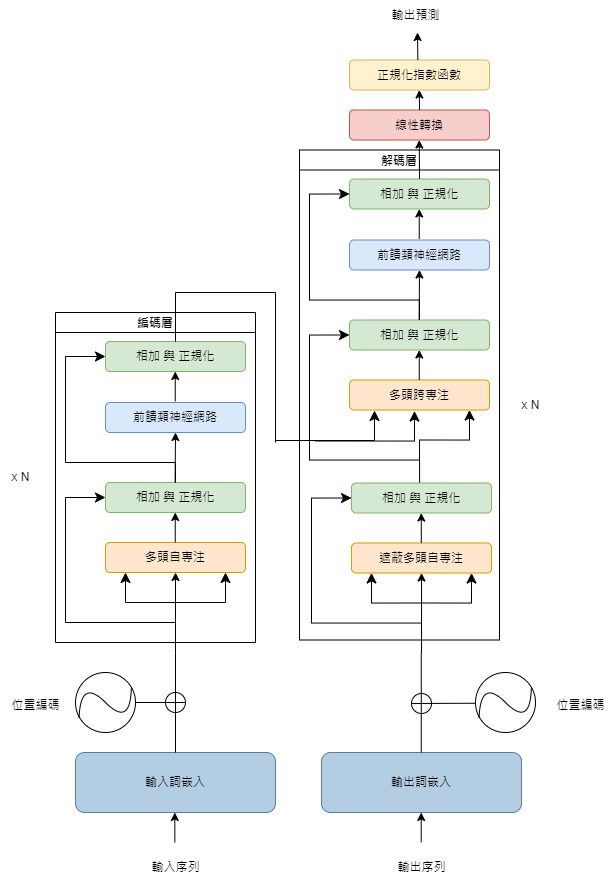
\includegraphics[width=0.9\linewidth]{figures/tfm_arch.drawio.png}
    \caption{轉換器架構圖}
    \label{fig:tfm_arch}
\end{figure}

        由於轉換器不需要對每個時間點逐一運算,使其得以實現高度平行化,類神經網路得以透過專注機制同時進行序列資料的大量訓練。這種可擴展性(Scalability)使其在自然語言和語音處理上取得了巨大的進展,幾乎取代了原先遞迴式類神經網路的應用場景,近年來甚至被應用在圖像類的資料上\cite{dosovitskiy2021image},展現了此種模型架構的彈性與泛用性,成為目前最前沿的人工智慧主流架構。

        除了模型架構,機器學習中不可或缺的另一大部分是對資料的編碼過程。如何更有效率的讓機器理解、處理和輸出資料,是機器學習乃至深層學習的一大課題。面對捉摸不定、抽象且變化萬千的人類語言,語音和文字處理中的表徵學習尤為重要。

\section{表徵與自監督式學習}

\subsection{特徵抽取與表徵學習}

  不論採用何種模型,為了讓機器可以處理並捕捉輸入資料中的訊號與模式(Pattern),包括如何對資料編碼和運算的步驟,在機器學習中稱之為特徵抽取(Feature Extraction)或表徵學習(Representation Learning),這是模型建構中不可或缺的重要步驟。

        對於抽象的語言概念,早期工程領域根據對語音和文字的理解,分別進行了不同的處理。對於離散且可計數的文字,人們使用詞頻統計衍生出如 n 連詞(n-gram)、TF-IDF(Term-Frequency Inverse Document Frequency)等特徵作為模型學習的前處理步驟;而對於連續且複雜的語音,工程師則透過聲學原理與訊號處理的知識,使用如濾波器組(Filter Bank)、梅爾倒頻譜係數(Mel-Frequency Cepstrum Coefficient,MFCC)等特徵,類比人耳捕捉語音訊號的過程。

        在深層學習逐漸發展的過程中,自然語言處理領域的一大里程碑是米氏(Mikolov)提出的「word2vec」模型 \cite{mikolov_efficient_2013},該模型以連續的向量表徵(Vector Representation)取代稀疏(Sparse)的統計數據,對離散的文字單詞進行「詞嵌入(Word Embedding)」編碼。通過大量文本運算,將各單詞之間的共現(Collocation)以跳躍詞(Skip-gram)、連續詞袋(Continuous Bag-of-Word,CBOW)等演算法轉換成高維向量空間中的點,找出每個單詞最適合的語義表徵。爾後,為了更細緻地捕捉同一單詞在不同句子中的脈絡變化,ELMo(Embeddings from Language Model)\cite{peters_deep_2018} 提出了「含上下文詞嵌入(Contextualized Embedding)」的概念,使得各單詞在運算表徵的過程中可以根據上下文進行些微調整。

\subsection{自監督學習}

  隨著轉換器模型的提出,BERT(來自轉換器的雙向編碼器表徵,Bidirectional Encoder Representations from Transformers)\cite{devlin_bert_2019} 被提出。通過自專注機制,工程師們無需依賴人工標記,透過預先設定任務(Pretext Task)引導模型從大量文本中自行找出更細緻且考量前後文(Contextualized)的語義關係,並在許多文字任務上獲得了優異的成績。

        自此,楊氏(LeCun)將這種以特定任務作為引導、藉助資料本身的結構替代標註,從大量未標註資料中進行學習資料模式(Pattern)的訓練方式,稱之為「自監督學習(Self-supervised Learning,SSL)」。BERT 的成功使自監督學習得以大行其道,並出現了許多由巨量資料進行預訓練(Pre-train)的基石模型(Foundation Model),有效解決了語言處理領域中的標註資料稀缺的問題。人們在解決語言相關任務時,不需從頭蒐集資料與進行耗時耗能的訓練過程,而是可以利用基石模型優良的泛化(Generalization)能力,解決各種應用任務的需求。相比於預訓練的任務,這些更貼近日常現實的任務被稱為「下游任務(Downstream Task)」,能應對廣泛的下游任務種類,這是基石模型最大的優勢。

        有鑑於文字處理方面的成功,語音領域的研究者嘗試將相似模式應用於語音,眾多語音基石模型隨之出現。大量的語音資料庫幫助模型萃取出有助於下游任務的語音表徵(Speech Representation),在各種任務上獲得了優於傳統聲學特徵的表現。語音表徵具備的無窮潛力,逐漸成為聲學特徵之外的新選擇。

        依照這些語音自監督模型的預訓練學習模式,可大致分為重建式、預測式與對比式模型。以下分別介紹這三類模式:

\subsubsection{重建式學習(Reconstruction Learning)}

  此類模型通過對輸入訊號進行擾動(Perturb)後,期望模型將被更動的輸入重新預測回原始資料,通常減損函數表示為:
\begin{align}
    \mathcal{L}_{recon} = \mathbb{E}_x[|f_\theta(\tilde{x}) - x|]
\end{align}
其中 $\tilde{x}$ 為擾動後的資料,$f_\theta(\cdot)$ 為模型函數。擾動方式通常以遮蔽為主,在文字處理中以 BERT 為代表,稱為「遮蔽語言模型(Masked Language Model,MLM)」。在語音中,採用此方式學習的有 Mockingjay \cite{liu_mockingjay_2019}、TERA \cite{t_tera_2021} 等模型。  % NPC

\subsubsection{預測式學習(Predictive Learning)}

  此類模型通過預訂一些學習目標函數,製造類似輸入與輸出的配對資料,讓模型預測該函數的結果來學習資料中的特定結構。其訓練減損函數可表示為:
\begin{align}
    \mathcal{L}_{pred} = \mathbb{E}_x[\text{eval}(f_\theta(x), \hat{f}(x))]
\end{align}
其中 $\hat{f}$ 是期望模型學習的目標函數,$f_\theta(\cdot)$ 為模型函數,$\text{eval}$ 是用來評估預測好壞的標準。

        目標函數的典型代表是自迴歸(Autoregressive),期望模型預測未來時間點的輸入表徵。文字方面以生成式預訓練轉換器(Generative Pretrained Transformer,GPT)系列 \cite{radford_language_nodate, brown_language_2020}為代表,語音上的自迴歸預測編碼(Autoregressive Predictive Coding,APC) \cite{chung_generative_2020} 也是採用此種模式。此外,語音基石模型還可以使用其他訓練目標,如 PASE+ \cite{ravanelli_multi-task_2020} 預測其他模型的表徵,而本文著重探究的「隱藏單元 BERT(Hidden-unit BERT,HuBERT)」\cite{hsu_hubert_2021, hsu_hubert_2021-2} 則以預測分群(Cluster)後的輸入表徵為目標,這些預測目標又被視為虛擬標註(Pseudo-label),後文將著重探討。

\subsubsection{對比式學習(Contrastive Learning)}

  此學習方式的訓練目標是要求模型區分正樣本(Positive Sample)與負樣本(Negative Sample)的差異,減損函數通常定義為:
\begin{align}
    \mathcal{L}_{contr} = -\mathbb{E}_x\left[\log
        \left(
        {\frac
            {\sum_{\tilde{x} \in x_{pos}}\exp(\text{sim}(x, \tilde{x}))}
            {\sum_{\tilde{x} \in \mathcal{X}}\exp(\text{sim}(x, \tilde{x}))}
        }\right)\right]
\end{align}

        其中 $x$ 為輸入,$x_{pos}$ 為正樣本,$\mathcal{X}$ 為包含正負樣本的資料集,$\text{sim}(\cdot, \cdot)$ 是評估兩個樣本相似程度的函數,常用的相似度函數為內積運算得出的餘弦相似度(Cosine Similarity)。語音上最早使用對比式學習的模型為對比預測編碼(Contrastive Predictive Coding,CPC)\cite{maekaku2022speech},之後如 Wav2vec \cite{schneider2019wav2vec}、Modified CPC \cite{rivière2020unsupervised}、Wav2vec 2.0 \cite{baevski2020wav2vec} 等模型亦是以對比正負樣本的模式訓練,但訓練時正負樣本的定義有所差異,如 Wav2vec 僅以時間維度上相同的向量為正樣本,其餘則將固定時間內的向量皆視為正樣本。

        對比式學習通過正負樣本的定義,將預訓練任務形塑為分類問題,因此減損函數本質上為交叉熵,使模型能夠判斷訓練資料中的結構差異。

\subsection{向量量化與離散單元}

  語音訊號雖然記錄語言資訊,卻與影像資料一樣都是連續數值資料,不像離散的文字較易處理,因此發展出了許多應用廣泛的模型。為了使語音模型訓練可以套用自然語言處理領域的演算法,從連續語音中找出離散表徵逐漸成為研究趨勢,這類研究被稱為「聲學單元發掘(Acoustic Unit Discovery,AUD)」。

        由於語言概念本質上是離散符號,向量量化技術常用於涉及語言標註的情境,如電腦視覺經典的量化向量變分自編碼器(Vector-Quantized Variational Autoencoder,VQ-VAE)\cite{van2017neural},利用影像標註的離散語言單詞特性,使模型學習的表徵向量被約束在編碼簿(Codebook) 的幾個向量中。

        在語音領域,基於 Wav2vec 之上的 Vq-wav2vec \cite{baevski2019vq} 和 Wav2vec 2.0 將連續的語音特徵量化加入訓練目標中,在語音辨識等任務上取得了顯著進步。

        HuBERT \cite{hsu_hubert_2021-2} 則先對連續的 MFCC 特徵進行 K-平均(K-Means)演算法分群,以所得的群心(Centroid)或碼字(Code Word)編號作為訓練目標,實施類似 BERT 的遮蔽語言模型訓練,並改以此次訓練得到的語音表徵為目標,再次分群後實施第二次訓練。這些經過兩輪訓練後,從模型表徵分群得到的群心,被視為「隱藏單元(Hidden Unit)」,呈現了語音訊號中的代表性聲學特徵。透過找出隱藏單元的過程,HuBERT 在低資源情況下達到與 Wav2vec 2.0 相近的語音辨識成績。

\subsection{無文字(Textless)架構}

  奠基於 HuBERT 等語音基石模型的成功,利用隱藏單元的概念,將大量語音資料表徵進行 K-平均演算法,作為這些語音訊號的虛擬標註。如此得到的大量離散隱藏單元形成了「虛擬文字(Pseudo-text)」的語料庫,基於這些離散單元訓練的語言模型,稱為「生成式口語語言模型(Generative Spoken Language Model,GSLM)」\cite{lakhotia_generative_2021-1}。配合反向語音合成訓練基於離散單元的語音生成模型,整體架構完全不依賴文字標註,訓練出純語音語言模型,稱為「無文字(Textless)架構」\cite{noauthor_textless_2021}。

        無文字模式在語音問答(Spoken Question Answering)\cite{lin2022dual}和語音到語音翻譯 (Speech-to-speech Translation)\cite{chen_speech--speech_2023}中取得了前所未有的進展。這些「離散單元(Discrete Unit)」被視為類似文字卻不依賴人類文字標記的語音表徵,具有儲存位元率低和可套用文字語言模型訓練模式的優勢,受到語音社群的廣泛借鑑,後續也帶出了許多如\cite{zhang2024speechtokenizer} 等將語音以離散表徵編碼的研究。

        雖然在系統與應用任務上取得了成功,但這些離散單元本身與文字的差異,及其對語音語言模型訓練的幫助,仍是領域內探討的焦點。有鑑於此,本論文基於語言知識,從最接近文字且與語音訊號最相關的「音位(Phoneme)」開始探討,期望了解離散單元能帶來的特徵及其對後續應用的幫助。

\section{本章節總結}

  本章節首先介紹了深層學習模型的核心部件 --- 類神經網路的基本原理,隨後對本論文研究的核心 --- 「語音表徵」與「離散單元」的發展與歷史進行了梳理。接下來的章節將緊扣這些基石模型得到的離散特徵,對其與「音位」這類語音學標記之間的統計關係進行更深入分析。


\setcounter{page}{23}
\mychcnt{3}  %
\section{相關研究}  

\subsection{無文字與離散語音表徵}

  自 HuBERT 帶起的研究之後,出現了愈來愈多離散表徵相關的研究,例如 \cite{10097097, abdullah23_interspeech, chang_exploration_2023, liu2024dinosr, zhang2024speechtokenizer, huang2023repcodec} 等等。它們在提出自己的離散表徵時,也會採取 HuBERT 的衡量方式,來驗證這些離散單元與語音中的內容及人類對語音的詮釋之間具有一定程度的相關性,並從資訊理論(Information Theory)的角度,證明這些離散單元確實具備區分不同語音資訊的能力。

\subsection{語音學分析}

  由於語音處理本身最終是針對人類語音,因此有一群研究者通過對人類語音的理解,將這些知識應用在分析模型如何對語音訊號建構表徵之上。例如 \cite{deseyssel22_interspeech, wells_phonetic_2022, 10097097, abdullah23_interspeech} 等研究。\par
        基於這些作品對語音離散表徵的興趣和探討,本論文也先透過過往幾個常用來分析語音表徵的方式,特別是HuBERT \cite{hsu_hubert_2021-2} 提出的標準進行初步的分析。


\section{分析結果}

\subsection{基於各自音位的分析}
\begin{table}[!htbp]
    \centering
    \begin{subtable}[t]{\textwidth}
        \centering
        \begin{tabular}{|c|c|c|c|c|c|} \hline
                        & 音位純度   & 分群純度   & 音位熵    & 離散單元熵  & PNMI   \\ \hline
            HuBERT      & 0.5256 & 0.3382 & 3.3152 & 3.8681 & 0.4993 \\ \hline    %% 1.6552 h
            Wav2vec 2.0 & 0.4006 & 0.2676 & 3.3152 & 3.8215 & 0.3706 \\ \hline    %% 1.2286 w
            CPC         & 0.5188 & 0.3812 & 3.3146 & 3.7918 & 0.4992 \\ \hline    %% 1.6545 c
            LogMel      & 0.3253 & 0.1473 & 3.3158 & 3.8630 & 0.2647 \\ \hline    %% 0.8776 l 
        \end{tabular}
        \caption{群數 = 50}
        \label{tab:ch3-clu050-phn}
    \end{subtable}

    \vspace{0.5cm}

    \begin{subtable}[t]{\textwidth}
        \centering
        \begin{tabular}{|c|c|c|c|c|c|} \hline
                        & 音位純度   & 分群純度   & 音位熵    & 離散單元熵  & PNMI   \\ \hline
            HuBERT      & 0.6097 & 0.2553 & 3.3152 & 4.5704 & 0.5786 \\ \hline    %% 1.9181 h
            Wav2vec 2.0 & 0.4877 & 0.2118 & 3.3152 & 4.5284 & 0.4596 \\ \hline    %% 1.5235 w
            CPC         & 0.5895 & 0.2674 & 3.3146 & 4.5034 & 0.5557 \\ \hline    %% 1.8418 c
            LogMel      & 0.3348 & 0.0931 & 3.3158 & 4.5591 & 0.2789 \\ \hline    %% 0.9247 l 
        \end{tabular}
        \caption{群數 = 100}
        \label{tab:ch3-clu100-phn}
    \end{subtable}

    \vspace{0.5cm}

    \begin{subtable}[t]{\textwidth}
        \centering
        \begin{tabular}{|c|c|c|c|c|c|} \hline
                        & 音位純度   & 分群純度   & 音位熵    & 離散單元熵  & PNMI   \\ \hline
            HuBERT      & 0.6474 & 0.1644 & 3.3152 & 5.2681 & 0.6289 \\ \hline    %% 2.0849 h
            Wav2vec 2.0 & 0.5427 & 0.1467 & 3.3152 & 5.2173 & 0.5188 \\ \hline    %% 1.7199 w
            CPC         & 0.6098 & 0.1789 & 3.3146 & 5.1885 & 0.5882 \\ \hline    %% 1.9497 c
            LogMel      & 0.3474 & 0.0569 & 3.3158 & 5.2322 & 0.2955 \\ \hline    %% 0.9798 l 
        \end{tabular}
        \caption{群數 = 200}
        \label{tab:ch3-clu200-phn}
    \end{subtable}

    \caption{不同群數在四種基石模型的音位分析數據}
    \label{tab:single-cluster-results}
\end{table}
  由表 \ref{tab:single-cluster-results} 中可以看出,分群的群數愈多時,音位的純度確實有所上升,但這可能是犧牲分群純度得來的。因此再看 PNMI 的指標可以發現,整體離散單元和音位標註的相關性還是有所提升的。此外,從不同模型來觀察,HuBERT 的表現是四種語音表徵中最好的,一定程度上可以證實 HuBERT 在找出語音中有意義單位上的效能,及其為什麼無文字架構通常以 HuBERT 作為抽取語音離散表徵的模型。

\subsection{基於語音學分類的分析}
\begin{table}[!htbp]
    \centering
    \begin{subtable}[t]{\textwidth}
        \centering
        \begin{tabular}{|c|c|c|c|c|c|} \hline
                        & 標註純度   & 分群純度   & 標註熵    & 離散單元熵  & NMI    \\ \hline
            HuBERT      & 0.7466 & 0.1422 & 1.7530 & 3.8681 & 0.5742 \\ \hline    %% h  1.0065
            Wav2vec 2.0 & 0.6913 & 0.1570 & 1.7530 & 3.8215 & 0.4682 \\ \hline    %% w  0.8208
            CPC         & 0.7418 & 0.1953 & 1.7530 & 3.7918 & 0.5644 \\ \hline    %% c  0.9894
            LogMel      & 0.5980 & 0.0953 & 1.7530 & 3.8630 & 0.3403 \\ \hline    %% l  0.5966 
        \end{tabular}
        \caption{群數 = 50}
        \label{tab:ch3-clu050-pcls}
    \end{subtable}

    \vspace{0.2cm}

    \begin{subtable}[t]{\textwidth}
        \centering
        \begin{tabular}{|c|c|c|c|c|c|} \hline
                        & 標註純度   & 分群純度   & 標註熵    & 離散單元熵  & NMI    \\ \hline
            HuBERT      & 0.7804 & 0.0856 & 1.7530 & 4.5704 & 0.6148 \\ \hline    %% h  1.0778
            Wav2vec 2.0 & 0.7219 & 0.0889 & 1.7530 & 4.5284 & 0.5252 \\ \hline    %% w  0.9207
            CPC         & 0.7790 & 0.0997 & 1.7530 & 4.5034 & 0.6046 \\ \hline    %% c  1.0599
            LogMel      & 0.6032 & 0.0567 & 1.7530 & 4.5591 & 0.3512 \\ \hline    %% l  0.6157 
        \end{tabular}
        \caption{群數 = 100}
        \label{tab:ch3-clu100-pcls}
    \end{subtable}

    \vspace{0.2cm}

    \begin{subtable}[t]{\textwidth}
        \centering
        \begin{tabular}{|c|c|c|c|c|c|} \hline
                        & 標註純度   & 分群純度   & 標註熵    & 離散單元熵  & NMI    \\ \hline
            HuBERT      & 0.8004 & 0.0464 & 1.7530 & 5.2681 & 0.6563 \\ \hline    %% h  1.1504
            Wav2vec 2.0 & 0.7490 & 0.0527 & 1.7530 & 5.2173 & 0.5671 \\ \hline    %% w  0.9941
            CPC         & 0.7947 & 0.0644 & 1.7530 & 5.1885 & 0.6345 \\ \hline    %% c  1.1123
            LogMel      & 0.6107 & 0.0335 & 1.7530 & 5.2322 & 0.3652 \\ \hline    %% l  0.6401 
        \end{tabular}
        \caption{群數 = 200}
        \label{tab:ch3-clu200-pcls}
    \end{subtable}

    \caption{不同群數在四種基石模型按照語音學類別的分析數據}
    \label{tab:single-cluster-phonetype-results}
\end{table}
  將表 \ref{tab:single-cluster-phonetype-results} 與音位的表 \ref{tab:single-cluster-results} 進行比較,能看出音位數據表現的趨勢,也能在語音類別中看出來。然而,由於語音類別數明顯少於音位的種類數,因此語音類別標註的純度相較音位會較高。

\setcounter{section}{4}
\section{分析結果}

\begin{figure}
    \centering
    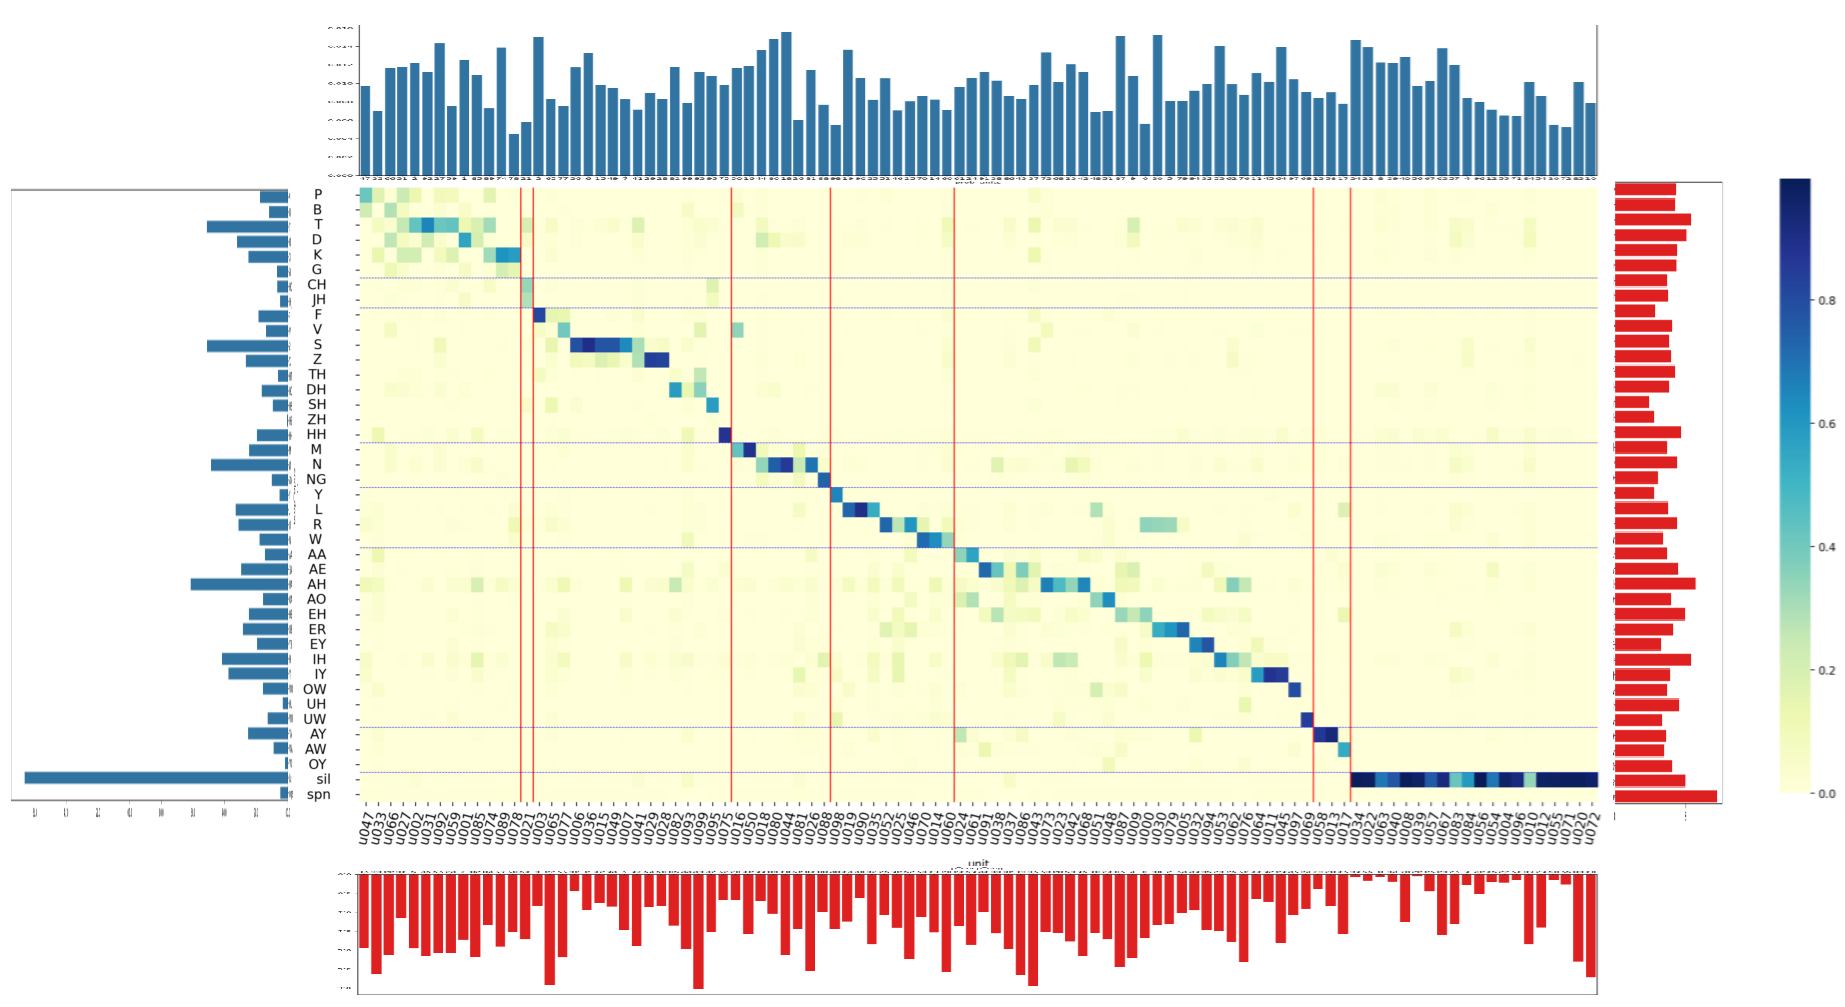
\includegraphics[width=1\linewidth]{figures/better__p_ph_given_un.png}
    \caption{HuBERT 100}
    \label{p_p_given_u-hub-100}
\end{figure}

  為了更直觀的了解模型離散單元與音素之間的對應關係,接下來的分析將把音素與單元的聯合分佈 \(p(p|u)\) 作圖呈現,如 \ref{p_p_given_u-hub-100} 所示。以下說明這張圖表的看法:\par
       橫軸是各單元,而縱軸是各音素,按照發音分組方式,輔音遵循國際音標的圖表排列,元音則按照 ARPABET (cite CMU Dict) 字母順序排列。由於離散單元編號本身並無特殊含義,因此當單元數太多時將省略。\par
       為了更好的看出各組別之間的關係,圖表上先將各組之間以橫線區分。按照語音學分組後,為了考慮單元之間的代表性,將每個單元都找出相對應最高機率的音素,接著將每個單元亦依照對應音素在縱軸的排列順序一一排列,若是遇到對應同一音素的兩種離散單元,則以 \(p(u|p) \) 由高至低排列。最後再橫軸上也以語音學分組區分。\par
       如此一來,便能夠呈現出一張由左上至右下的對應圖。這張圖在 (cite DinoSR) 等 paper 也有呈現。從圖中可以看出,用來編碼 sil 的 unit 其實佔據了不小的部分。

% 
\chapter{多個語音離散表徵與音位的關係}

\textcolor{red}{tokenization 的翻譯需要調整!}

\section{動機}

  如前一章所述,一個文字或音位往往對應到上百毫秒的語音訊號,然而單一離散單元所對應的聲音訊號為 10 或 20 毫秒,亦即同一段語音所對應的離散單元數目將比音位或文字多出許多。本章節從自然語言處理中獲取靈感,將分詞演算法(Tokenization)應用於離散單元序列上,並應用上一章節的分析方法檢驗將多個離散單元所組成之符記。探討分詞後,離散單元是否可以同時擁有無文字(Textless)\cite{lakhotia_generative_2021, lakhotia_generative_2021-1, noauthor_textless_2021} 的特性,且更接近音位的序列,成為更好的語音表徵。

\section{相關研究} 

  在無文字架構被提出後的約兩年後,藉分詞方法組合離散單元的研究逐步出現。最初提出「聲學片段(Acoustic Piece)」的是任氏(Ren)等人 \cite{ren_speech_2022}\citetag{1-22A4-Pretrain-ap}),該論文比對離散單元序列及對應的文字轉寫,從中觀察到許多相似的模式(Pattern),而且不限於單一語者。受此啟發,本論文首先將離散單元使用句子片段(SentencePiece) \cite{kudo_sentencepiece_2018} 分詞,獲得新的符記 --- 「聲學片段(Acoustic Piece)」,並用於語音辨識的預訓練上。

        不久,由吳氏(Wu)提出的 Wav2seq \cite{wu_wav2seq_2023}\citetag{2-22A5-wav2seq}論文中,考量文字與語音的序列長度差異,並基於離散單元和音位的關聯性,將離散單元視為字符(Character),嘗試將這些字符透過分詞方法組成「虛擬語言(Pseudo-language\footnote{偽語言對應之離散單元被視為「虛擬文字(Pseudo-text)」})」,來幫助語音到文字的模型。因為解碼器在實際應用時需要生成的序列多是文字的符記 --- 次詞單位(Subword Unit),因此該篇研究旨在讓模型在預訓練後可以快速適應下游任務。與前一篇呼應,「聲學片段」對語音預訓練的效果在\cite{10096788}\citetag{3-23A-coarser-grain}中被探討,此後聲學片段更被應用於縮短資料序列長度\cite{chang_exploration_2023}\citetag{4-23B-Exploration of Efficient End-to-End ASR using Discretized Input from Self-Supervised Learning} 、語音生成\cite{shen2024acoustic}\citetag{5-24A-speech-gen},或學習更穩健(Robust)的語音表徵\cite{chang2023r}\citetag{6-23B-rspin-acousticpiece}。

        近期,張氏(Chang)等人\cite{chang_exploring_2024}\citetag{7-23B-shinji-hsiuhsuan}將以分詞方法處理離散單元的流程(Pipeline)納入 ESPNet 套件 \cite{watanabe2018espnet} 中,並在語音辨識、語音翻譯等任務中獲得了超越以往的表現,進一步證明了這個方法的效果。

\section{分詞方法}

  在以文字為主體的自然語言處理中,文字文本除了以單詞(Word)或字元(Character)為處理單位,更常見的作法是透過分詞演算法(Tokenization)將文本分段,以「次詞單位(Subword Unit)」構成詞彙表來重新編碼文本,用於文字模型的訓練與推理。

        分詞方法的優點一般包含:

\begin{enumerate}
    \item 固定詞彙表大小,避免未登錄詞(Out-of-vocabulary,OOV)
    \item 縮短資料序列的長度,提升訓練和推論的效率。
    \item 分解單詞,捕捉更細緻的語意關係,模擬如英語中的字首(Prefix)、字尾(Suffix)等等具有特定意義的文字組合。
\end{enumerate}

\subsection{常見演算法}

  以下介紹幾種常見的分詞方法:

\paragraph{位元組對編碼(Byte Pair Encoding,BPE)}\hfill \break

  位元組對編碼 \cite{10.5555/177910.177914, sennrich_neural_2016} 是一種常用的分詞方法,最初來自資料壓縮技術 \cite{10.5555/177910.177914},後來被引入到自然語言處理領域,用以處理機器翻譯問題 \cite{sennrich_neural_2016} 。
該演算法從字元開始,根據詞彙表中各個次詞單位的頻率,反覆合併常見的字元成為新的次詞單位,直到達到預定的詞彙表大小。

\paragraph{單詞片段(WordPiece)}\hfill \break

  WordPiece \cite{wu2016google} 演算法由 Google 用以訓練機器翻譯系統,並在 BERT \cite{devlin_bert_2019} 模型中被使用而廣為人知。與 BPE 同樣是透過反覆合併的策略,但合併的依據改以機率模型取代出現頻率。

\paragraph{單一詞語言模型(Unigram Language Model)}\hfill \break

  單一詞語言模型 \cite{kudo2018subword} 是基於語言模型的分詞方法,以機率分佈選擇次詞單位,並以最大化輸入文本的機率來為文本分段。

\subsection{句子片段(SentencePiece)套件}

  SentencePiece \cite{kudo_sentencepiece_2018}
是由 Google 開發的分詞套件,實作了前述的 BPE 和單一詞演算法。其優勢在於可應用於不同語言,尤其用於處理中文、日文等不使用空格分隔單詞的語言文本時,此套件大大的簡化了前處理的流程。

\section{衡量方式}

  本章節沿用上一章節 LibriSpeech 資料集的 train-clean-100 訓練子集,以及相同的分析數據以進行比對。由於與上一章節的差異僅在分詞方法的引入,因此數據結果將多紀錄分詞前後序列長度的變化;其他操控變因包含分詞方法與詞表大小。考慮到語音訊號本身不如英語等文字,在書寫時就已經具備空格分隔單詞,因此以下分析結果皆採用 SentencePiece 套件中實作之單一詞演算法為分詞方法,並比較詞表大小 500、1000、8000、10000、20000 五種設定的結果差異。(空間不足時則僅呈現 500、1000、10000 三種設定的趨勢。)

\section{分析結果}\newcommand{\jefftablesep}{\vspace{0.5cm}}\renewcommand{\arraystretch}{0.7} % 調整行高

    以下數據中的「長度壓縮比率」係指透過分詞方法後,每一個句子的「單詞」數與原先離散單元的數量相比之比值。由於長度壓縮比率是針對離散單元分詞所得到,與標註無關,因此只在音位分析的表格上呈現。

\subsection{基於各自音位的分析}

  首先,為了比較不同詞表大小對於純度、相互資訊等數據的影響,先分別固定語音模型為 HuBERT 和 Wav2vec 2.0,在離散單元的分群數量為 50、100、200 三種設定下,觀察詞表大小造成的變化。由 HuBERT (表 \ref{tab:hubert-phn-results})和 Wav2vec 2.0(表 \ref{tab:w2v2-phn-results})的數據比較可觀察到,詞表大小上升除了使得音位純度提高以外,相互資訊也是隨之提高的,可以發現使用分詞方法並給予足夠大的詞表,對於找出語音中的資訊確實有所幫助。

        接著從另一個角度切入,比較同樣都是離散單元分群數為 200 的條件下,不同語音基石模型的分析數據。由表 \ref{tab:ch4-models-phn} 可以發現,HuBERT 模型在音位純度與相互資訊勝過其他模型,這個結論與上一章節是一致的。

        有趣的是,觀察長度壓縮比率可以發現,CPC 模型在分詞演算法的引入後,能夠使序列變得最短,但同時在音位純度與相互資訊上也有所犧牲;而 HuBERT 雖然在這些分析數據上高過其他三者,卻同時達成了比 Wav2vec 2.0 和 LogMel 更好的壓縮比率。因此綜合看來,或許這是為什麼目前使用語音離散單元進行研究時,HuBERT 模型仍然是領域內的首選。

                
\begin{table}[!htbp]
    \centering
    \begin{subtable}[t]{\textwidth}
        \centering
        \begin{tabular}{|c|c|c|c|c|c|c|} \hline 
                詞表大小  & 音位純度 & 分群純度 & 音位熵 & 離散單元熵 &    PNMI & 長度壓縮比率 \\ \hline 
50 (未分詞)& 0.5256& 0.3382& 3.3152& 3.8681& 0.4993&1.0000\\ \hline 
                   500  &   0.5574   &  0.0829 &   3.3152  &  6.0282 & 0.5357 & 0.3486  \\ \hline %%  1.7758       
                  1000  &   0.5744   &  0.0556 &   3.3152  &  6.6594 & 0.5466 & 0.2992  \\ \hline %%  1.8120       
                  8000  &   0.5957   &  0.0257 &   3.3152  &  8.5192 & 0.5729 & 0.2074  \\ \hline %%  1.8993       
                 10000  &   0.5955   &  0.0238 &   3.3152  &  8.7207 & 0.5750 & 0.2007  \\ \hline %%  1.9063       
                 20000  &   0.5921   &  0.0182 &   3.3152  &  9.3527 & 0.5820 & 0.1819  \\ \hline %%  1.9293       
        \end{tabular}
\caption{群數 = 50}
        \label{tab:ch4-hubert-phn-clu050}
    \end{subtable}        

    \jefftablesep        

    \begin{subtable}[t]{\textwidth}
        \centering
        \begin{tabular}{|c|c|c|c|c|c|c|} \hline 
                詞表大小  & 音位純度 & 分群純度 & 音位熵 & 離散單元熵 &    PNMI & 長度壓縮比率 \\ \hline 
100 (未分詞)& 0.6097& 0.2553& 3.3152& 4.5704& 0.5786&1.0000\\ \hline 
                   500  &   0.6260   &  0.0972 &   3.3152  &  6.0655 & 0.5990 & 0.4432  \\ \hline %%  1.9858       
                  1000  &   0.6372   &  0.0631 &   3.3152  &  6.7181 & 0.6089 & 0.3666  \\ \hline %%  2.0186       
                  8000  &   0.6536   &  0.0237 &   3.3152  &  8.5954 & 0.6308 & 0.2444  \\ \hline %%  2.0912       
                 10000  &   0.6527   &  0.0219 &   3.3152  &  8.7938 & 0.6324 & 0.2357  \\ \hline %%  2.0965       
                 20000  &   0.6490   &  0.0173 &   3.3152  &  9.4123 & 0.6378 & 0.2123  \\ \hline %%  2.1145       
        \end{tabular}
\caption{群數 = 100}
        \label{tab:ch4-hubert-phn-clu100}
    \end{subtable}        

    \jefftablesep        

    \begin{subtable}[t]{\textwidth}
        \centering
        \begin{tabular}{|c|c|c|c|c|c|c|} \hline 
                詞表大小  & 音位純度 & 分群純度 & 音位熵 & 離散單元熵 &    PNMI & 長度壓縮比率 \\ \hline 
200 (未分詞)& 0.6474& 0.1644& 3.3152& 5.2681& 0.6289&1.0000\\ \hline 
                   500  &   0.6471   &  0.0930 &   3.3152  &  6.0986 & 0.6314 & 0.5995  \\ \hline %%  2.0934       
                  1000  &   0.6540   &  0.0558 &   3.3152  &  6.7786 & 0.6382 & 0.4609  \\ \hline %%  2.1156       
                  8000  &   0.6690   &  0.0208 &   3.3152  &  8.6544 & 0.6567 & 0.2874  \\ \hline %%  2.1769       
                 10000  &   0.6693   &  0.0189 &   3.3152  &  8.8535 & 0.6584 & 0.2764  \\ \hline %%  2.1826       
                 20000  &   0.6684   &  0.0144 &   3.3152  &  9.4737 & 0.6636 & 0.2467  \\ \hline %%  2.1999      
        \end{tabular}
\caption{群數 = 200}
        \label{tab:ch4-hubert-phn-clu200}
    \end{subtable}        

\caption{HuBERT 模型在不同詞表大小時的音位分析數據}
    \label{tab:hubert-phn-results}
\end{table}



\begin{table}[!htbp]
    \centering
    \begin{subtable}[t]{\textwidth}
        \centering
        \begin{tabular}{|c|c|c|c|c|c|c|} \hline 
                詞表大小  & 音位純度 & 分群純度 & 音位熵 & 離散單元熵 &    PNMI & 長度壓縮比率 \\ \hline 
 50 (未分詞)&  0.4006 &   0.2676 & 3.3152 &     3.8215 & 0.3706&1.0000\\ \hline 
                  500  &   0.4295&     0.0594    &3.3152 &   6.0328  &       0.4027 &0.3943 \\ \hline %%  
                 1000  &   0.4411&     0.0456    &3.3152 &   6.6250  &       0.4132 &0.3448 \\ \hline %%  
                 8000  &   0.4676&     0.0239    &3.3152 &   8.4954  &       0.4438 &0.2429 \\ \hline %%  
                10000  &   0.4705&     0.0227    &3.3152 &   8.6966  &       0.4477 &0.2352 \\ \hline %%  
                20000  &   0.4753&     0.0185    &3.3152 &   9.3471  &       0.4587 &0.2132 \\ \hline %%  
        \end{tabular}
\caption{群數 = 50}
        \label{tab:ch4-w2v2-phn-clu050}
    \end{subtable}        

    \jefftablesep        

    \begin{subtable}[t]{\textwidth}
        \centering
        \begin{tabular}{|c|c|c|c|c|c|c|} \hline 
                詞表大小  & 音位純度 & 分群純度 & 音位熵 & 離散單元熵 &    PNMI & 長度壓縮比率 \\ \hline 
 100 (未分詞)&0.4877 &   0.2118 & 3.3152 &     4.5284 & 0.4596&1.0000\\ \hline 
                  500  &   0.5016&     0.0697    &3.3152 &   6.0769  &       0.4784 &0.4926 \\ \hline %%  
                 1000  &   0.5108&     0.0444    &3.3152 &   6.7265  &       0.4867 &0.4160 \\ \hline %%  
                 8000  &   0.5427&     0.0215    &3.3152 &   8.5576  &       0.5180 &0.2895 \\ \hline %%  
                10000  &   0.5451&     0.0203    &3.3152 &   8.7602  &       0.5218 &0.2797 \\ \hline %%  
                20000  &   0.5531&     0.0162    &3.3152 &   9.4070  &       0.5345 &0.2526 \\ \hline %%  
        \end{tabular}
\caption{群數 = 100}
        \label{tab:ch4-w2v2-phn-clu100}
    \end{subtable}        

    \jefftablesep        

    \begin{subtable}[t]{\textwidth}
        \centering
        \begin{tabular}{|c|c|c|c|c|c|c|} \hline 
                詞表大小  & 音位純度 & 分群純度 & 音位熵 & 離散單元熵 &    PNMI & 長度壓縮比率 \\ \hline 
 200 (未分詞)&  0.5427 &   0.1467 & 3.3152 &     5.2173 & 0.5188 &1.0000\\ \hline 
                  500  &   0.5481&     0.0846    &3.3152 &   6.0756  &       0.5276 &0.6418 \\ \hline %%  
                 1000  &   0.5549&     0.0509    &3.3152 &   6.7483  &       0.5347 &0.5178 \\ \hline %%  
                 8000  &   0.5803&     0.0180    &3.3152 &   8.6065  &       0.5632 &0.3498 \\ \hline %%  
                10000  &   0.5828&     0.0166    &3.3152 &   8.8136  &       0.5668 &0.3373 \\ \hline %%  
                20000  &   0.5917&     0.0129    &3.3152 &   9.4561  &       0.5794 &0.3026  \\ \hline %%  
        \end{tabular}
\caption{群數 = 200}
        \label{tab:ch4-w2v2-phn-clu200}
    \end{subtable}        

\caption{Wav2vec 2.0 模型在不同詞表大小時的音位分析數據}
    \label{tab:w2v2-phn-results}
\end{table}




\begin{table}[!htbp]
    \centering
    \begin{subtable}[t]{\textwidth}
        \centering
        \begin{tabular}{|c|c|c|c|c|c|c|} \hline 
                詞表大小  & 音位純度 & 分群純度 & 音位熵 & 離散單元熵 &    PNMI & 長度壓縮比率 \\ \hline 
200 (未分詞)&   0.6474 &   0.1644 & 3.3152 &     5.2681 & 0.6289 &1.0000\\ \hline 
                    500   & 0.6471   & 0.0930   & 3.3152 &  6.0986    &  0.6314 &  0.5995  \\ \hline %%   2.0934
                   1000   & 0.6540   & 0.0558   & 3.3152 &  6.7786    &  0.6382 &  0.4609  \\ \hline %%   2.1156
                  10000   & 0.6693   & 0.0189   & 3.3152 &  8.8535    &  0.6584 &  0.2764  \\ \hline %%   2.1826
        \end{tabular}
\caption{HuBERT}
        \label{tab:ch4-phn-model-hubert}
    \end{subtable}        

    \jefftablesep        

    \begin{subtable}[t]{\textwidth}
        \centering
        \begin{tabular}{|c|c|c|c|c|c|c|} \hline 
                詞表大小  & 音位純度 & 分群純度 & 音位熵 & 離散單元熵 &    PNMI & 長度壓縮比率 \\ \hline 
200 (未分詞)&   0.5427 &   0.1467 & 3.3152 &     5.2173 & 0.5188 &1.0000\\ \hline 
                    500   & 0.5481   & 0.0846   & 3.3152 &  6.0756    &  0.5276 &  0.6418  \\ \hline %%   1.7491
                   1000   & 0.5549   & 0.0509   & 3.3152 &  6.7483    &  0.5347 &  0.5178  \\ \hline %%   1.7727
                  10000   & 0.5828   & 0.0166   & 3.3152 &  8.8136    &  0.5668 &  0.3373  \\ \hline %%   1.8791
        \end{tabular}
\caption{Wav2vec 2.0}
        \label{tab:ch4-phn-model-w2v2}
    \end{subtable}        

    
    \jefftablesep        

    \begin{subtable}[t]{\textwidth}
        \centering
        \begin{tabular}{|c|c|c|c|c|c|c|} \hline 
                詞表大小  & 音位純度 & 分群純度 & 音位熵 & 離散單元熵 &    PNMI & 長度壓縮比率 \\ \hline 
200 (未分詞)&   0.6098 &   0.1789 & 3.3146 &     5.1885 & 0.5882 &1.0000\\ \hline 
                    500   & 0.6116   & 0.1048   & 3.3146 &  6.0343    &  0.5936 &  0.4951  \\ \hline %%   1.9677
                   1000   & 0.6134   & 0.0618   & 3.3146 &  6.7245    &  0.5979 &  0.3523  \\ \hline %%   1.9818
                  10000   & 0.6198   & 0.0171   & 3.3146 &  8.8593    &  0.6118 &  0.2061  \\ \hline %%   2.0277
        \end{tabular}
\caption{CPC}
        \label{tab:ch4-phn-model-cpc}
    \end{subtable}        

    \jefftablesep        

    \begin{subtable}[t]{\textwidth}
        \centering
        \begin{tabular}{|c|c|c|c|c|c|c|} \hline 
                詞表大小  & 音位純度 & 分群純度 & 音位熵 & 離散單元熵 &    PNMI & 長度壓縮比率 \\ \hline 
200 (未分詞)&   0.3474 &   0.0569 & 3.3158 &     5.2322 & 0.2955 &1.0000\\ \hline 
                    500   & 0.3515   & 0.0403   & 3.3158 &  6.1035    &  0.3066 &  0.6304  \\ \hline %%   1.0166
                   1000   & 0.3547   & 0.0228   & 3.3158 &  6.7602    &  0.3129 &  0.5185  \\ \hline %%   1.0376
                  10000   & 0.3699   & 0.0121   & 3.3158 &  8.7579    &  0.3381 &  0.3427  \\ \hline %%   1.1211
        \end{tabular}
\caption{LogMel}
        \label{tab:ch4-phn-model-logmel}
    \end{subtable}        

\caption{固定離散單元群數皆為 200,不同基石模型的音位分析數據}
    \label{tab:ch4-models-phn}
\end{table}


\subsection{基於語音學分類的分析}

  最後觀察將語音標註換成語音學分類的結果,一樣可以從表 \ref{tab:hubert-pcls-results}、\ref{tab:w2v2-pcls-results} 和 \ref{tab:ch4-models-pcls} 觀察到與上一小節相同的趨勢。

                
        \begin{table}[!htbp]
            \centering
            \begin{subtable}[t]{\textwidth}
                \centering
                \begin{tabular}{|c|c|c|c|c|c|} \hline 
                        詞表大小  & 標註純度 & 分群純度 & 標註熵 & 離散單元熵 &     NMI   \\ \hline 
                       50 (未分詞)&   0.7466  &  0.1422 & 1.7530 &   3.8681 &  0.5742 \\ \hline 
                           500    &  0.7510  &  0.0345  & 1.7530 &  6.0282  &     0.5789  \\ \hline 
                          1000    &  0.7492  &  0.0225  & 1.7530 &  6.6594  &     0.5756  \\ \hline 
                          8000    &  0.7288  &  0.0116  & 1.7530 &  8.5192  &     0.5630  \\ \hline 
                         10000    &  0.7248  &  0.0110  & 1.7530 &  8.7207  &     0.5606  \\ \hline 
                         20000    &  0.7109  &  0.0089  & 1.7530 &  9.3527  &     0.5537  \\ \hline 
                \end{tabular}
\caption{群數 = 50}
                \label{tab:ch4-hubert-pcls-clu050}
            \end{subtable}        

            \jefftablesep        

            \begin{subtable}[t]{\textwidth}
                \centering
                \begin{tabular}{|c|c|c|c|c|c|} \hline 
                        詞表大小  & 標註純度 & 分群純度 & 標註熵 & 離散單元熵 &     NMI   \\ \hline 
 100 (未分詞)&              0.7804 &   0.0856 &         1.7530 &     4.5704 &  0.6148\\ \hline 
                           500    &  0.7787  &  0.0300  & 1.7530 &  6.0655  &     0.6178  \\ \hline 
                          1000    &  0.7751  &  0.0210  & 1.7530 &  6.7181  &     0.6176  \\ \hline 
                          8000    &  0.7507  &  0.0095  & 1.7530 &  8.5954  &     0.6030  \\ \hline 
                         10000    &  0.7468  &  0.0087  & 1.7530 &  8.7938  &     0.6008  \\ \hline 
                         20000    &  0.7347  &  0.0072  & 1.7530 &  9.4123  &     0.5943  \\ \hline 
                \end{tabular}
\caption{群數 = 100}
                \label{tab:ch4-hubert-pcls-clu100}
            \end{subtable}        

            \jefftablesep        

            \begin{subtable}[t]{\textwidth}
                \centering
                \begin{tabular}{|c|c|c|c|c|c|} \hline 
                        詞表大小  & 標註純度 & 分群純度 & 標註熵 & 離散單元熵 &     NMI   \\ \hline 
 200 (未分詞)&              0.8004 &   0.0464 &         1.7530 &     5.2681 &  0.6563\\ \hline 
                           500    &  0.7875  &  0.0269  & 1.7530 &  6.0986  &     0.6469  \\ \hline 
                          1000    &  0.7788  &  0.0170  & 1.7530 &  6.7786  &     0.6385  \\ \hline 
                          8000    &  0.7625  &  0.0071  & 1.7530 &  8.6544  &     0.6266  \\ \hline 
                         10000    &  0.7601  &  0.0064  & 1.7530 &  8.8535  &     0.6251  \\ \hline 
                         20000    &  0.7514  &  0.0051  & 1.7530 &  9.4737  &     0.6200   \\ \hline
                \end{tabular}
\caption{群數 = 200}
                \label{tab:ch4-hubert-pcls-clu200}
            \end{subtable}        

\caption{HuBERT 模型在不同詞表大小時的語音學類別分析數據}
            \label{tab:hubert-pcls-results}
        \end{table}

\begin{table}[!htbp]
    \centering
    \begin{subtable}[t]{\textwidth}
        \centering
        \begin{tabular}{|c|c|c|c|c|c|} \hline 
                詞表大小 & 標註純度 & 分群純度 & 標註熵 & 離散單元熵 &     NMI \\ \hline 
 50 (未分詞)&      0.6913 &   0.1570 &         1.7530 &     3.8215 &  0.4682\\ \hline 
                  500  &  0.7018 &    0.0339 &   1.7530 &   6.0328 &       0.4873  \\ \hline 
                 1000  &  0.7058 &    0.0273 &   1.7530 &   6.6250 &       0.4913  \\ \hline 
                 8000  &  0.7041 &    0.0158 &   1.7530 &   8.4954 &       0.4956  \\ \hline 
                10000  &  0.7033 &    0.0152 &   1.7530 &   8.6966 &       0.4963  \\ \hline 
                20000  &  0.6961 &    0.0128 &   1.7530 &   9.3471 &       0.4954  \\ \hline 
        \end{tabular}
\caption{群數 = 50}
        \label{tab:ch4-w2v2-pcls-clu050}
    \end{subtable}        

    \jefftablesep        

    \begin{subtable}[t]{\textwidth}
        \centering
        \begin{tabular}{|c|c|c|c|c|c|} \hline 
                詞表大小 & 標註純度 & 分群純度 & 標註熵 & 離散單元熵 &     NMI \\ \hline 
 100 (未分詞)&     0.7219 &   0.0889 &         1.7530 &     4.5284 &  0.5252 \\ \hline 
                  500  &  0.7142 &    0.0288 &   1.7530 &   6.0769 &       0.5297  \\ \hline 
                 1000  &  0.7132 &    0.0197 &   1.7530 &   6.7265 &       0.5294  \\ \hline 
                 8000  &  0.7173 &    0.0108 &   1.7530 &   8.5576 &       0.5352  \\ \hline 
                10000  &  0.7171 &    0.0105 &   1.7530 &   8.7602 &       0.5360  \\ \hline 
                20000  &  0.7149 &    0.0089 &   1.7530 &   9.4070 &       0.5379  \\ \hline 
        \end{tabular}
\caption{群數 = 100}
        \label{tab:ch4-w2v2-pcls-clu100}
    \end{subtable}        

    \jefftablesep        

    \begin{subtable}[t]{\textwidth}
        \centering
        \begin{tabular}{|c|c|c|c|c|c|} \hline 
                詞表大小 & 標註純度 & 分群純度 & 標註熵 & 離散單元熵 &     NMI \\ \hline 
  200 (未分詞)&     0.7490 &   0.0527 &         1.7530 &     5.2173 &  0.5671  \\ \hline 
                  500  &  0.7465 &    0.0310 &   1.7530 &   6.0756 &       0.5685  \\ \hline 
                 1000  &  0.7451 &    0.0199 &   1.7530 &   6.7483 &       0.5692  \\ \hline 
                 8000  &  0.7405 &    0.0071 &   1.7530 &   8.6065 &       0.5725  \\ \hline 
                10000  &  0.7399 &    0.0066 &   1.7530 &   8.8136 &       0.5729  \\ \hline 
                20000  &  0.7391 &    0.0055 &   1.7530 &   9.4561 &       0.5757   \\ \hline
        \end{tabular}
\caption{群數 = 200}
        \label{tab:ch4-w2v2-pcls-clu200}
    \end{subtable}        

\caption{Wav2vec 2.0 模型在不同詞表大小時的語音學類別分析數據}
    \label{tab:w2v2-pcls-results}
\end{table}


        \begin{table}[!htbp]
            \centering
            \begin{subtable}[t]{\textwidth}
                \centering
                \begin{tabular}{|c|c|c|c|c|c|} \hline 
                        詞表大小  & 標註純度 & 分群純度 & 標註熵 & 離散單元熵 &     NMI  \\ \hline 
  200 (未分詞)&         0.8004 &   0.0464 &         1.7530 &     5.2681 &  0.6563\\ \hline 
                            500 &  0.7875 &    0.0269 &   1.7530   & 6.0986 &    0.6469 \\ \hline %%   2.0934
                           1000 &  0.7788 &    0.0170 &   1.7530   & 6.7786 &    0.6385 \\ \hline %%   2.1156
                          10000 &  0.7601 &    0.0064 &   1.7530   & 8.8535 &    0.6251 \\ \hline %%   2.1826
                \end{tabular}
\caption{HuBERT}
                \label{tab:ch4-pcls-model-hubert}
            \end{subtable}        

            \jefftablesep        

            \begin{subtable}[t]{\textwidth}
                \centering
                \begin{tabular}{|c|c|c|c|c|c|} \hline 
                        詞表大小  & 標註純度 & 分群純度 & 標註熵 & 離散單元熵 &     NMI  \\ \hline 
  200 (未分詞)&         0.7490 &   0.0527 &         1.7530 &     5.2173 &  0.5671 \\ \hline 
                            500 &  0.7465 &    0.0310 &   1.7530   & 6.0756 &    0.5685 \\ \hline %%   1.7491
                           1000 &  0.7451 &    0.0199 &   1.7530   & 6.7483 &    0.5692 \\ \hline %%   1.7727
                          10000 &  0.7399 &    0.0066 &   1.7530   & 8.8136 &    0.5729 \\ \hline %%   1.8791
                \end{tabular}
\caption{Wav2vec 2.0}
                \label{tab:ch4-pcls-model-w2v2}
            \end{subtable}        

            
            \jefftablesep        

            \begin{subtable}[t]{\textwidth}
                \centering
                \begin{tabular}{|c|c|c|c|c|c|} \hline 
                        詞表大小  & 標註純度 & 分群純度 & 標註熵 & 離散單元熵 &     NMI  \\ \hline 
 200 (未分詞)&         0.7947 &   0.0644 &         1.7530 &     5.1885 &  0.6345 \\ \hline 
                            500 &  0.7925 &    0.0369 &   1.7530   & 6.0343 &    0.6368 \\ \hline %%   1.9677
                           1000 &  0.7882 &    0.0223 &   1.7530   & 6.7245 &    0.6349 \\ \hline %%   1.9818
                          10000 &  0.7609 &    0.0096 &   1.7530   & 8.8593 &    0.6175 \\ \hline %%   2.0277
                \end{tabular}
\caption{CPC}
                \label{tab:ch4-pcls-model-cpc}
            \end{subtable}        

            \jefftablesep        

            \begin{subtable}[t]{\textwidth}
                \centering
                \begin{tabular}{|c|c|c|c|c|c|} \hline 
                詞表大小 & 標註純度 & 分群純度 & 標註熵 & 離散單元熵 &     NMI \\ \hline 
  200 (未分詞)&         0.6107 &   0.0335 &         1.7530 &     5.2322 &  0.3652 \\ \hline 
                            500 &  0.6156 &    0.0247 &   1.7530   & 6.1035 &    0.3801 \\ \hline %%   1.0166
                           1000 &  0.6189 &    0.0137 &   1.7530   & 6.7602 &    0.3875 \\ \hline %%   1.0376
                          10000 &  0.6322 &    0.0096 &   1.7530   & 8.7579 &    0.4085 \\ \hline %%   1.1211
                \end{tabular}
\caption{LogMel}
                \label{tab:ch4-pcls-model-logmel}
            \end{subtable}        

\caption{固定離散單元群數皆為 200,不同基石模型的語音學類別分析數據}
            \label{tab:ch4-models-pcls}
        \end{table}
        


\section{本章總結}

  藉由分詞演算法的引入,我們可以發現在序列長度相對縮短的前提下,音位的純度卻也獲得了提升,足以證明分詞演算法的引入,可以幫助離散單元考量多於一個音框的語音資訊,建構於精細的音框之上,找出更接近人類解讀語音最小單位資訊。期望以此發現,可以使得語音語言模型建立時,模型在處理語音語料庫時,能夠以更接近文字的序列長度與資訊進行訓練,獲得更接近文字模型的效果。

% \chapter{結論與展望}

\section{研究貢獻與討論}
  
本論文的主旨,在於分析語音基石模型的離散表徵,與語音標註之間的純度和相互資訊等數據的相關性,並且透過分詞方法的引入,嘗試將多個離散單元進行結合後,觀察學習到的新符記是否和音位等標註更加一致。 

首先,論文第三章介紹了與無文字架構以及語音表徵相關的分析研究,隨後簡介語音學知識中,對於不同音位之間如何按照發音特性分門別類。有了音位與語音學分類兩種語音標註後,借鑑 HuBERT 提及的純度和相互資訊的分析方式,對離散表徵與語音標註之間,兩者的相關性進行分析與觀察,比對無文字架構中不同語音離散表徵的統計特性。結果可發現,HuBERT 作為目前無文字架構最常用的語音離散表徵模型的理由,很可能來自於它們的音位純度與相互資訊都相對較高,因而更能捕捉到語音中與內容相關的重要資訊,且同樣的趨勢在語音學分類的標註也可以被觀察到。

其後在論文第四章,考慮到音位與離散單元往往是一對多的關係,
藉著嘗試引入自然語言處理常用的分詞方法,
重新對離散單元的序列進行分組,並且比較不同詞表大小對這些分析數據的影響。
考量語音不如英語的文字系統具備明確的空格提示,
本研究採取單一詞作為分詞方法進行
實驗,
並比較不同模型與不同詞表大小對第三章的分析數據是否造成影響。

結果顯示,
藉助加入分詞方法並提供足夠大的詞表,確實能夠讓不同音位的純度以及相互資訊有所提升,
讓多個離散單元之間有機會相互結合、重新分組,更能捕捉語音訊號中的內容資訊。
且在四種語音表徵之間,HuBERT 依然是所有模型中音位純度和相互資訊最高者,還達成了一定的序列長度壓縮比率,相較之下 CPC 模型雖然壓縮比率更低,卻犧牲掉過多語音資訊導致相關數據反而較差。這也解釋了為什麼目前在離散單元相關的研究中,無論是使用單一離散單元,或是使用分詞方法進行長度壓縮等,HuBERT 都仍是最有利於後續語音任務的訓練與應用的模型。

 

\section{未來展望}
  
希望這些對離散單元與分詞方法應用的嘗試,能幫助我們在訓練任務之前,決定哪種語音基石模型更適合作為離散編碼語音訊號的基礎。接下來,我們期望能針對常見的語音任務,特別是語音辨識和語音翻譯等內容處理相關的任務,比對離散單元促成的實際成效和分析數據之間的關係,並對這些任務中的錯誤案例進行統計和個案探討。

另外,對於如何結合語音離散單元,除了將其視為文字進行分詞演算法外,我們還可以使用其他方式對離散單元序列進行分組,以達成壓縮序列長度並使其與音位等語音內容更加一致的目標。例如,將此目標形塑為語音分段(Speech Segmentation)任務等,也是未來可以嘗試的離散單元分組方式。

最後,利用語音學分組的切入點,或許可以在未來分析離散單元或連續語音表徵時,不再僅限於參考音位或文字,還可以從語音學知識提供的相似性資訊出發,為錯誤發音修正等任務提供衡量的依據。

